\chapter{Introduction Générale et État de l'Art en Recherche Visuelle}
\label{chap:intro_etat_art}

\section{Contexte Institutionnel et Problématique}

L'avènement exponentiel des technologies de numérisation, des capteurs photographiques haute résolution et des plateformes multimédias a engendré une prolifération massive de données visuelles non structurées. Face à des corpus photographiques se chiffrant en dizaines de milliers d'unités, les paradigmes traditionnels d'indexation textuelle manuelle se heurtent à une impossibilité matérielle et cognitive manifeste.

Dans ce contexte scientifique et technologique stimulant, le présent projet de fin d'études s'inscrit dans le cadre du cursus de Master en Génie Informatique dispensé à la \textbf{Faculté des Sciences et Techniques de Tanger (FSTT)}, affiliée à l'\textbf{Université Abdelmalek Essaâdi}, au titre de l'année universitaire 2026--2027. Les travaux consignés dans ce rapport ont été confiés au \textbf{Groupe 13}, avec pour mission thématique d'excellence l'étude, la conception et la réalisation de la méthode d'\textbf{Estimation de la Pertinence des Descripteurs} (\textit{Feature Relevance Estimation} -- FRE) appliquée à la recherche d'images par le contenu.

\subsection{Du Texte au Contenu Visuel}
Pendant plusieurs décennies, la recherche iconographique a reposé sur l'indexation par mots-clés ou descriptions textuelles. Bien qu'intuitive, cette approche souffre de limitations structurelles~:
\begin{enumerate}[label=\bfseries\alph*.]
    \item \textbf{Subjectivité et polysémie~:} La description textuelle dépend de la sensibilité et de la langue de l'opérateur. Deux observateurs qualifieront une même teinte ou un motif abstrait de manière divergente.
    \item \textbf{Coût prohibitif~:} L'étiquetage exhaustif de corpus volumineux requiert un investissement humain colossal, incompatible avec les flux d'ingestion modernes.
    \item \textbf{Critères intrinsèquement visuels~:} Trouver une texture rugueuse similaire, une harmonie de teintes ou un motif géométrique spécifique constitue une tâche qu'aucun mot du dictionnaire ne saurait encapsuler avec la précision du pixel.
\end{enumerate}

La \textbf{recherche par le contenu visuel} (\textit{Content-Based Image Retrieval}) propose une alternative radicale~: interroger une collection d'images directement à partir de son essence visuelle intrinsèque. Néanmoins, une difficulté théorique centrale émerge~: le \textbf{fossé sémantique} (\textit{semantic gap}).

\begin{infobox}{Définition : Le Fossé Sémantique (Semantic Gap)}
Le fossé sémantique désigne l'écart irrémédiable existant entre les informations numériques élémentaires pouvant être extraites des données matricielles (valeurs de pixels, contrastes locaux, gradients) et l'interprétation sémantique, contextuelle et affective qu'un être humain associe à cette même scène visuelle~\cite{smeulders2000content}.
\end{infobox}

\section{Fondements de la Recherche par Similarité Visuelle}

Le postulat mathématique de la recherche d'images par similarité visuelle consiste à modéliser chaque image sous la forme d'un vecteur multidimensionnel $\mathbf{x} \in \mathbb{R}^D$ résumant son contenu visuel, puis à évaluer la proximité visuelle entre deux images au moyen d'une fonction de similarité $S(\mathbf{x}_i, \mathbf{x}_j) \in [0, 1]$.

Dans les systèmes conventionnels d'indexation visuelle, les signatures visuelles sont structurées en deux grandes familles canoniques~:
\begin{itemize}
    \item \textbf{Descripteurs de Couleur~:} Les histogrammes HSV globaux modélisent la distribution des longueurs d'ondes de manière invariante aux translations et rotations~; les moments statistiques de Stricker \& Orengo~\cite{stricker1995similarity} capturent la moyenne, la variance et l'asymétrie spectrale~; et les palettes de couleurs dominantes résument les teintes majeures par partitionnement $K$-Means.
    \item \textbf{Descripteurs de Texture~:} Les matrices de co-occurrence de niveaux de gris (GLCM) de Haralick et al.~\cite{haralick1973textural} mesurent le contraste, la corrélation, l'énergie et l'homogénéité spatiale~; tandis que les motifs binaires locaux (LBP) d'Ojala et al.~\cite{ojala2002multiresolution} encodent la micro-texture locale invariante aux variations lumineuses monotones.
\end{itemize}

\section{Cahier des Charges et Démarche Méthodologique}

Le tableau~\ref{tab:objectifs_projet} synthétise le périmètre fonctionnel et technique assigné à la plateforme \textbf{Perceptra}.

\begin{table}[H]
\centering
\rowcolors{2}{LightGray}{white}
\begin{tabularx}{\textwidth}{>{\bfseries}p{3.5cm}X}
\toprule
\rowcolor{TableHeader}
\color{white}Axe Fonctionnel & \color{white}Objectifs \& Spécifications Clés \\
\midrule
Authentification \& Sessions & Contrôle d'accès par jetons JWT, isolation étanche des galeries par utilisateur et gestion des rôles (RBAC). \\
Gestion de Collection & Importation unitaire et par lots (batch), suppression sécurisée, détection des doublons par somme SHA-256 et favoris. \\
Organisation Hiérarchique & Arborescence personnalisable de catégories avec relations parent-enfant récursives et intégrité référentielle. \\
Studio de Transformation & Moteur de retouche non destructif (recadrage, redimensionnement interpolé, rotations, affines) préservant l'original. \\
Extraction Visuelle & Pipeline automatique de descripteurs normalisés de couleur (HSV 768-D, Moments 9-D, KMeans) et de texture (GLCM, LBP 256-D). \\
Moteur de Recherche Visuelle & Recherche par image requête avec calcul vectoriel multi-espaces, pondération convexe ajustable et ordonnancement Top-K. \\
Relevance Feedback FRE & Spécificité Groupe 13 : analyse de dispersion intra/inter-classe, critère de Fisher, mise à jour des poids et centroïde. \\
Évaluation Quantitative & Validation expérimentale sur \textbf{GHIM-10K} (10\,000 images) via les courbes de précision ($P@K$), rappel ($R@K$) et temps de calcul. \\
\bottomrule
\end{tabularx}
\caption{Synthèse des exigences du cahier des charges de Perceptra}
\label{tab:objectifs_projet}
\end{table}

Pour satisfaire ces exigences, le système déploie le pipeline fonctionnel unifié illustré sur la figure~\ref{fig:pipeline_fonctionnel}, reliant l'ingestion, la caractérisation déterministe, la recherche vectorielle et la boucle de rétroaction.

\begin{figure}[H]
\centering
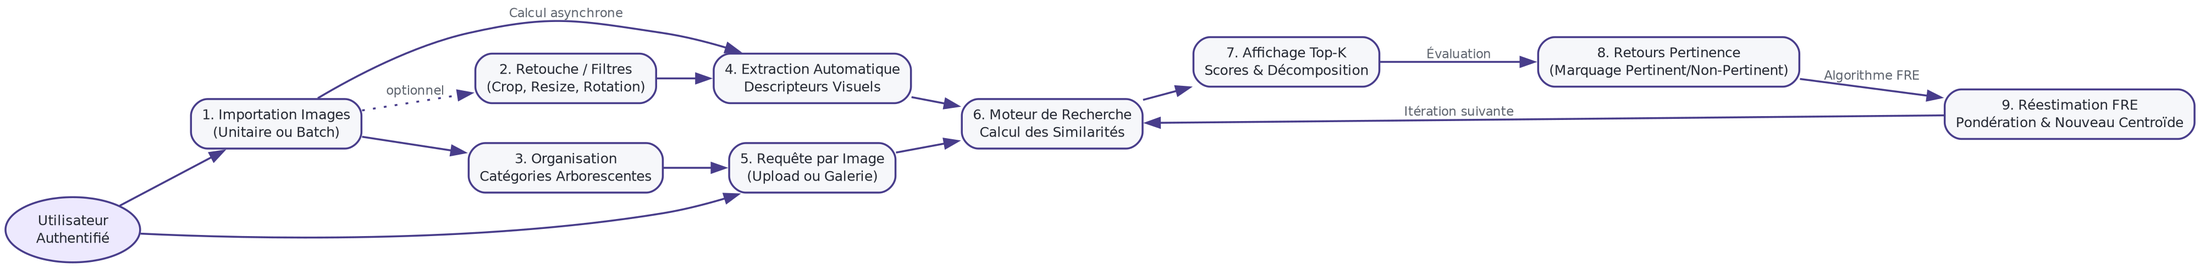
\includegraphics[width=0.60\textwidth]{images/01-perceptra-pipeline-fonctionnel.png}
\caption{Pipeline fonctionnel et parcours utilisateur au sein de Perceptra}
\label{fig:pipeline_fonctionnel}
\end{figure}
